\section{Modifying the annotation vocabulary and semantics}

Right-click the project file for which you want to modify the annotation semantics and open it with the \emph{Swproj Model Editor}.
There you can view or edit the EMF model objects that build up a \emph{Reprotool} project. Under the \emph{Software Project} tree node,
you can see the default \emph{Annotation Groups}, what \emph{annotations} and \emph{CTL formulas} they contain. By modifying these
formulas, you can modify the annotation semantics. You can also add new \emph{AnnotationGroups} to add custom annotations to the
\emph{Reprotool} project and to specify their semantics using the NuSMV \emph{CTL} or \emph{LTL} formulas.

\begin{figure}[ht]
  \centering
  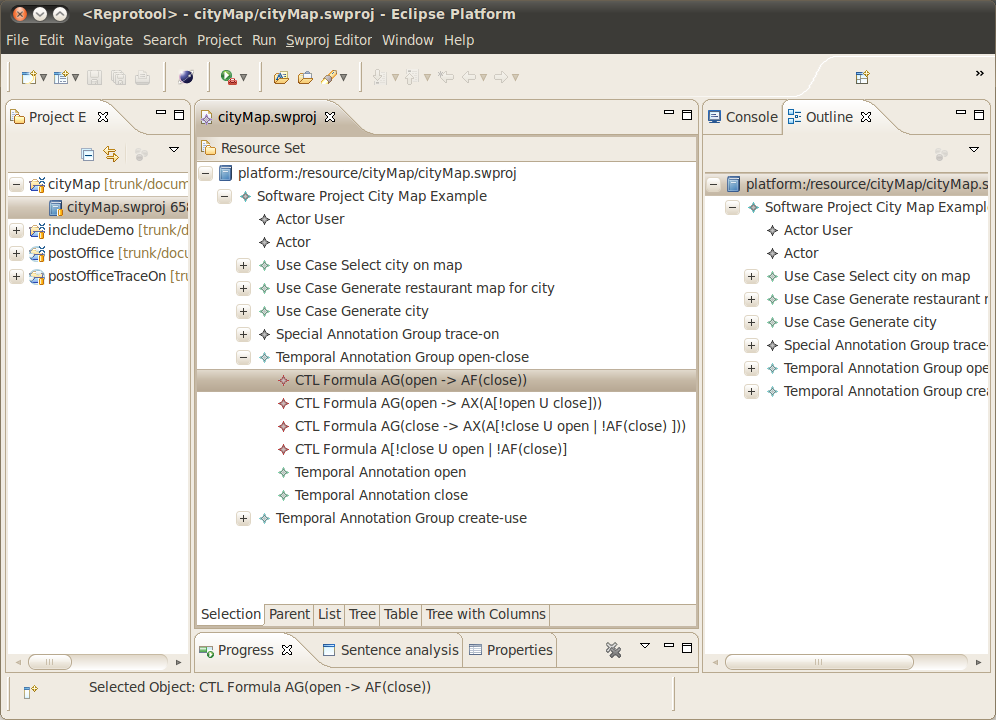
\includegraphics[height=280pt]{images/reprotoolCTLFormulas}
  \caption{The \emph{open-close} annotation group with annotations and default \emph{CTL} formulas}
  \label{fig:reprotoolCTLFormulas}
\end{figure}

\newpage

\subsection{Adding \emph{lock / unlock} annotations to a \emph{Reprotool} project}
Now we are going to show you how you can add new annotations to a \emph{Reprotool} project. We will add two annotations to our project.
These two annotations are \emph{lock} and \emph{unlock}. These two annotations will use the semantics of a recursive lock. More
precisly, the model checking in \emph{Reprotool} will check if there is an \emph{unlock} annotation present in every possible
execution path after the \emph{lock} annotation appears.

\subsubsection{Adding a new \emph{temporal annotation group} to the project}
First we need to add a new \emph{temporal annotation group} to our project. Open the project using \emph{Swproj Model Editor}.
Right-click on the \emph{Software project} tree node and select the \texttt{New Child / Temporal Annotation Group} command.
This will add a new \emph{temporal annotation group} to our project.

\subsubsection{Adding annotations to the \emph{temporal annotation group}.}
Now we are going to add the \emph{lock} and \emph{unlock} annotations to the newly-created annotation group. Right-click this annotation
group and select the command \texttt{New Child / Temporal Annotation}. Fill the annotation name as \emph{lock} in the properties
view. Use the same command to add the \emph{unlock} annotation to this annotation group.

\subsubsection{Adding semantics to the \emph{lock / unlock} annotations.}
Right-click the new \emph{Annotation group} in the \emph{Swproj Model Editor} and select the command \texttt{New Child / CTL Formula}
from the context menu. Now type \emph{After 'lock' there always needs to be 'unlock'} as the formula \emph{Description} in the
\emph{Properties view}. Type \texttt{AG(lock -> AF(unlock))} as \emph{Formula} in the \emph{Properties view}.
You should now be in a situation shown in the following figure:

\newpage

\begin{figure}[ht]
  \centering
  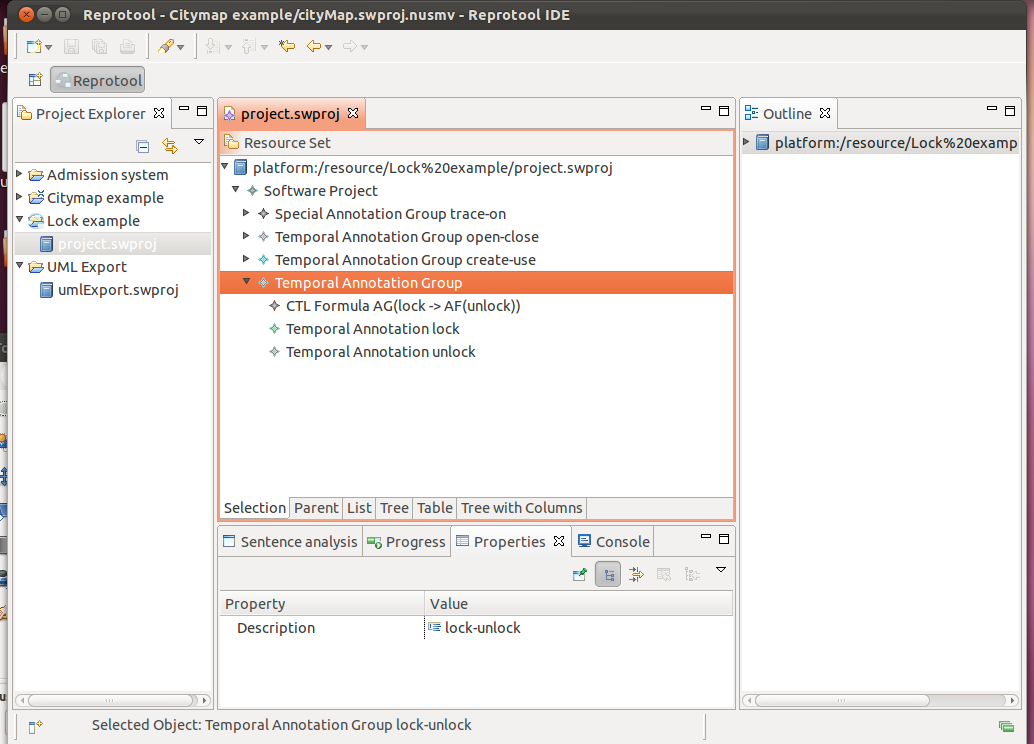
\includegraphics[height=280pt]{images/reprotoolLockUnlock}
  \caption{The new \emph{lock-unlock} annotation group}
  \label{fig:reprotoolLockUnlock}
\end{figure}

In the \emph{Reprotool} example projects, there is a project named \emph{Lock example}. We have added the \emph{lock / unlock}
annotations to this project. In the project, you can find a simple use-case that has a single execution path where the resources
are not properly unlocked. Running the model-cheking process on this example yields the expected result:

\begin{figure}[ht]
  \centering
  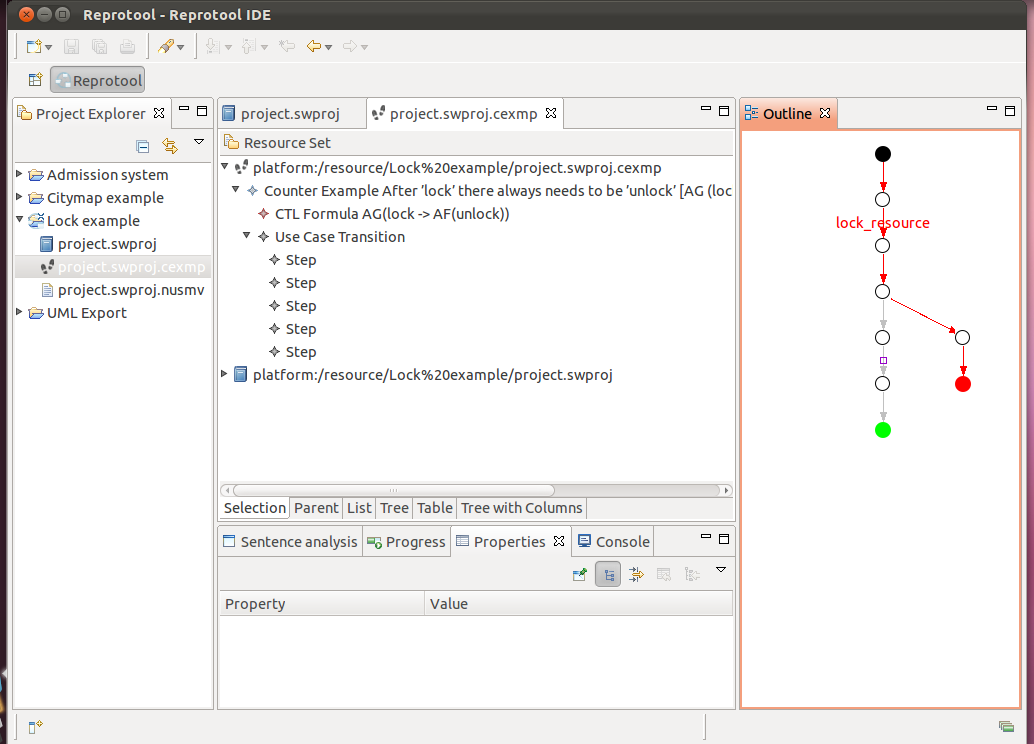
\includegraphics[height=280pt]{images/reprotoolLockUnlock2}
  \caption{The \emph{unlock} annotation is missing in this execution path}
  \label{fig:reprotoolLockUnlock2}
\end{figure}